\documentclass[a4paper,11pt]{article}
\input{/home/tof/Documents/Cozy/latex-include/preambule_doc.tex}
\input{/home/tof/Documents/Cozy/latex-include/preambule_commun.tex}
\newcommand{\showprof}{show them}  % comment this line if you don't want to see todo environment
\setlength{\fboxrule}{0.8pt}
\fancyhead[L]{\fbox{\Large{\textbf{Algo 05}}}}
\fancyhead[C]{\textbf{Exercies tris}}
\newdate{madate}{10}{09}{2020}
%\fancyhead[R]{\displaydate{madate}} %\today
\fancyhead[R]{Première - NSI}
\fancyfoot[L]{\vspace{1mm}Christophe Viroulaud}
\AtEndDocument{\label{lastpage}}
\fancyfoot[C]{\textbf{Page \thepage/\pageref{lastpage}}}
\fancyfoot[R]{\includegraphics[width=2cm,align=t]{/home/tof/Documents/Cozy/latex-include/cc.png}}

\begin{document}
\begin{exo}
En considérant que la durée d'exécution du tri par sélection est proportionnelle à $n^2$ et qu'il prend 6,8 secondes pour trier 16000 éléments, combien de temps prendra-t-il pour trier 1 million d'éléments?
\end{exo}
\begin{exo}
Le tri par insertion fait remonter l'élément en cours jusqu'à sa place, en effectuant des échanges de proche en proche.
\begin{center}
    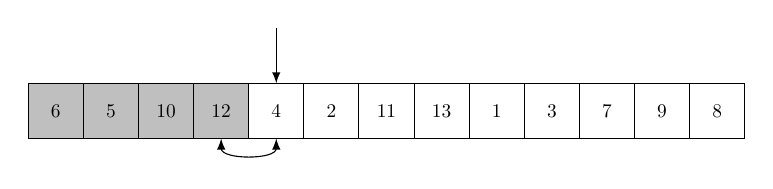
\begin{tikzpicture}[scale=0.7,transform shape]
        \draw[fill=gray!50] (0,0)--(4,0)--(4,1)--(0,1)--cycle;
        \draw (0,0) grid (13,1);
        \foreach \n/\x in {6/0,5/1,10/2,12/3,4/4,2/5,11/6,13/7,1/8,3/9,7/10,9/11,8/12}{
                \node (\n) at (0.5+\x,0.5) {\n};

            }

        \draw[->,>=latex] (4.5,2) -- (4.5,1);
        \draw[<->,>=latex] (3.5,0) to[bend right=90] (4.5,0);
    \end{tikzpicture}
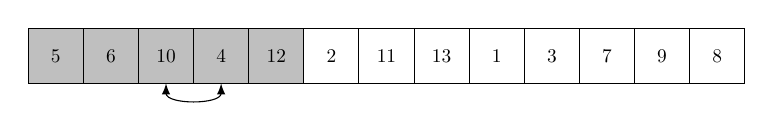
\begin{tikzpicture}[scale=0.7,transform shape]
    \draw[fill=gray!50] (0,0)--(5,0)--(5,1)--(0,1)--cycle;
    \draw (0,0) grid (13,1);

    \foreach \n/\x in {5/0,6/1,10/2,4/3,12/4,2/5,11/6,13/7,1/8,3/9,7/10,9/11,8/12}{
            \node (\n) at (0.5+\x,0.5) {\n};

        }
    \draw[<->,>=latex] (2.5,0) to[bend right=90] (3.5,0);
\end{tikzpicture}
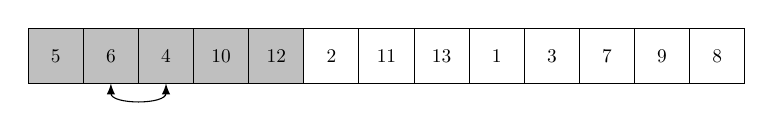
\begin{tikzpicture}[scale=0.7,transform shape]
    \draw[fill=gray!50] (0,0)--(5,0)--(5,1)--(0,1)--cycle;
    \draw (0,0) grid (13,1);

    \foreach \n/\x in {5/0,6/1,4/2,10/3,12/4,2/5,11/6,13/7,1/8,3/9,7/10,9/11,8/12}{
            \node (\n) at (0.5+\x,0.5) {\n};

        }
    \draw[<->,>=latex] (1.5,0) to[bend right=90] (2.5,0);
\end{tikzpicture}
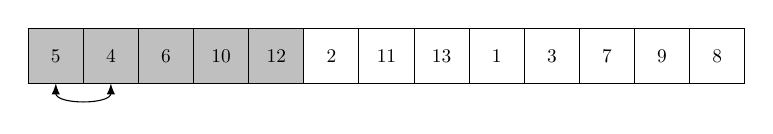
\begin{tikzpicture}[scale=0.7,transform shape]
    \draw[fill=gray!50] (0,0)--(5,0)--(5,1)--(0,1)--cycle;
    \draw (0,0) grid (13,1);

    \foreach \n/\x in {5/0,4/1,6/2,10/3,12/4,2/5,11/6,13/7,1/8,3/9,7/10,9/11,8/12}{
            \node (\n) at (0.5+\x,0.5) {\n};

        }
    \draw[<->,>=latex] (0.5,0) to[bend right=90] (1.5,0);
\end{tikzpicture}
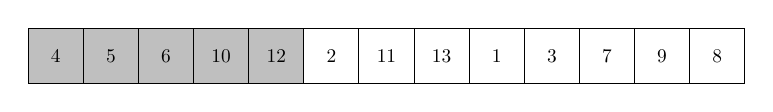
\begin{tikzpicture}[scale=0.7,transform shape]
    \draw[fill=gray!50] (0,0)--(5,0)--(5,1)--(0,1)--cycle;
    \draw (0,0) grid (13,1);

    \foreach \n/\x in {4/0,5/1,6/2,10/3,12/4,2/5,11/6,13/7,1/8,3/9,7/10,9/11,8/12}{
            \node (\n) at (0.5+\x,0.5) {\n};

        }
\end{tikzpicture}
\end{center}
Une autre méthode consiste à:
\begin{itemize}
    \item stocker l'élément en cours, 
    \item décaler vers la droite tous les éléments supérieurs,
    \item placer l'élément en cours à la bonne place.
\end{itemize}
\begin{center}
    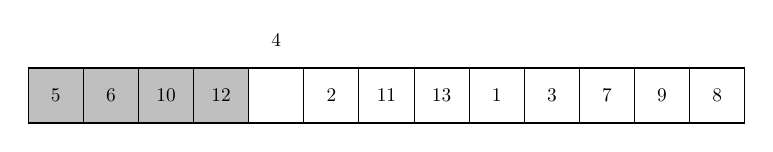
\begin{tikzpicture}[scale=0.7,transform shape]
        \draw[fill=gray!50] (0,0)--(4,0)--(4,1)--(0,1)--cycle;
        \draw (0,0) grid (13,1);
        \foreach \n/\x in {5/0,6/1,10/2,12/3, /4,2/5,11/6,13/7,1/8,3/9,7/10,9/11,8/12}{
                \node (\n) at (0.5+\x,0.5) {\n};

            }
            \node (4) at (4.5,1.5) {4};
    \end{tikzpicture}
    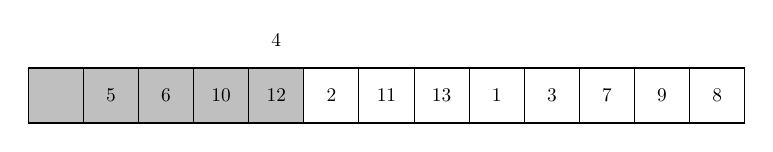
\begin{tikzpicture}[scale=0.7,transform shape]
        \draw[fill=gray!50] (0,0)--(5,0)--(5,1)--(0,1)--cycle;
        \draw (0,0) grid (13,1);
        \foreach \n/\x in {/0,5/1,6/2,10/3, 12/4,2/5,11/6,13/7,1/8,3/9,7/10,9/11,8/12}{
                \node (\n) at (0.5+\x,0.5) {\n};

            }
            \node (4) at (4.5,1.5) {4};
    \end{tikzpicture}
\end{center}
\begin{center}
    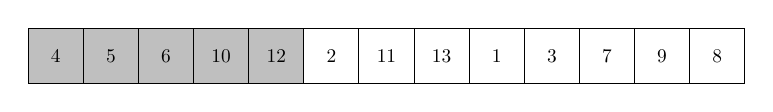
\begin{tikzpicture}[scale=0.7,transform shape]
        \draw[fill=gray!50] (0,0)--(5,0)--(5,1)--(0,1)--cycle;
        \draw (0,0) grid (13,1);
        \foreach \n/\x in {4/0,5/1,6/2,10/3, 12/4,2/5,11/6,13/7,1/8,3/9,7/10,9/11,8/12}{
                \node (\n) at (0.5+\x,0.5) {\n};

            }
    \end{tikzpicture}
\end{center}
Écrire la fonction \textbf{\texttt{tri\_insertion(tab: list) $\rightarrow$ None}} qui implémente ce nouvel algorithme.
\end{exo}
\begin{exo}
    On considère le tableau:
    \begin{lstlisting}[language=Python,basicstyle=\ttfamily\small, xleftmargin=2em, xrightmargin=2em]
[3, 4, 1, 7, 2]
\end{lstlisting}
Donner l'état du tableau après chaque itération quand on effectue: 
\begin{enumerate}
    \item un tri par sélection,
    \item un tri par insertion.
\end{enumerate}
\end{exo}
\begin{exo}
Pour comparer si deux tableaux de même longueur sont identiques, c’est-à-dire s'ils contiennent les mêmes éléments, une stratégie consiste à d'abord les trier puis comparer chaque élément un à un.
\begin{enumerate}
    \item Construire la fonction \textbf{\texttt{comparer(tab1: list, tab2: list) $\rightarrow$ bool}} qui compare les éléments des tableaux un à un et renvoie \textbf{\texttt{True}} s'ils sont identiques.
    \item Utiliser la fonction tri par insertion pour trier les tableaux:
    \begin{itemize}
        \item \textbf{\texttt{[3, 5, 9, 0, 1, 8, 2]}},
        \item \textbf{\texttt{[9, 5, 3, 2, 8, 1, 0]}}.
    \end{itemize}
    \item Comparer les deux tableaux avec la fonction \textbf{\texttt{comparer}}.
\end{enumerate}

\end{exo}
\begin{exo}
Le tri par insertion effectue un tri en place. Pour ne pas modifier les données initiales, il faut construire un nouveau tableau.
\begin{enumerate}
    \item Reprendre le tri de l'exercice 2 et écrire la fonction \textbf{\texttt{tri\_insertion(tab: list) $\rightarrow$ list}} qui crée un nouveau tableau trié à partir des éléments de \textbf{\texttt{tab}}. La fonction suivra l'algorithme suivant:
    \begin{itemize}
        \item parcourir \textbf{\texttt{tab}} et copier l'élément de rang \textbf{\texttt{i}} à la fin du nouveau tableau,
        \item insérer cet élément à la bonne position dans le nouveau tableau.
    \end{itemize} 
    \item Construire par compréhension un tableau de dix éléments aléatoires compris entre 0 et 100.
    \item Tester la fonction de tri sur ce tableau.
\end{enumerate}
\end{exo}
\begin{exo}
\begin{enumerate}
    \item Adapter le tri par insertion vu en cours pour trier le tableau de tuples suivants en fonction du premier élément des tuples:
    \begin{lstlisting}[language=Python, basicstyle=\ttfamily\small, xleftmargin=2em, xrightmargin=2em]
tab = [(5, "a"), (8, "b"), (1, "e"), (5, "d"), (7, "f"), (8, "c")]
\end{lstlisting}
    \item Un \emph{tri stable} conserve l'ordre relatif des éléments de même valeur. Le tri par insertion est-il stable?
\end{enumerate}
\end{exo}
\begin{exo}
\begin{enumerate}
    \item Construire par compréhension un tableau de cent éléments aléatoires compris entre 0 et 10.
    \item En s'aidant du tri par insertion, écrire la fonction \textbf{\texttt{max\_occurrences(tab: list) $\rightarrow$ int}} qui renvoie l'élément le plus présent dans le tableau. \underline{Indication:} dans un tableau trié les éléments identiques se suivent. 
\end{enumerate}
\end{exo}
\begin{exo}
Le tri à bulles \emph{fait remonter} les plus grands éléments d'un tableau, comme des bulles d'air qui remonteraient à la surface d'un liquide. Le code \ref{bulle} présente la première itération qui permet de propager le plus grand élément en dernière place du tableau. Il suffit ensuite d'effectuer une deuxième itération pour propager le deuxième plus grand élément en avant-dernière position.
    \begin{center}
        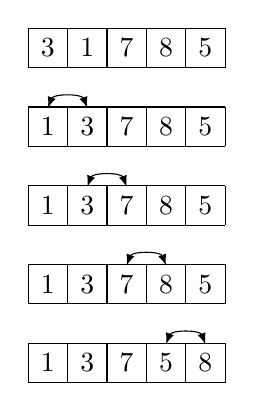
\begin{tikzpicture}[scale=0.5]
            \draw (0,0) grid (5,1);
            \node at(0.5,0.5) {3};
            \node at(1.5,0.5) {1};
            \node at(2.5,0.5) {7};
            \node at(3.5,0.5) {8};
            \node at(4.5,0.5) {5};

            
            \draw (0,-2) grid (5,-1);
            \node (1) at(0.5,-1.5) {1};
            \node (2)at(1.5,-1.5) {3};
            \node at(2.5,-1.5) {7};
            \node at(3.5,-1.5) {8};
            \node at(4.5,-1.5) {5};
            \draw[<->,>=latex] (1.north)to[bend left=70](2.north);

            \draw (0,-4) grid (5,-3);
            \node at(0.5,-3.5) {1};
            \node (3)at(1.5,-3.5) {3};
            \node (4)at(2.5,-3.5) {7};
            \node at(3.5,-3.5) {8};
            \node at(4.5,-3.5) {5};
            \draw[<->,>=latex] (3.north)to[bend left=70](4.north);

            \draw (0,-6) grid (5,-5);
            \node at(0.5,-5.5) {1};
            \node at(1.5,-5.5) {3};
            \node (5)at(2.5,-5.5) {7};
            \node (6)at(3.5,-5.5) {8};
            \node at(4.5,-5.5) {5};
            \draw[<->,>=latex] (5.north)to[bend left=70](6.north);
    
            \draw (0,-8) grid (5,-7);
            \node at(0.5,-7.5) {1};
            \node at(1.5,-7.5) {3};
            \node at(2.5,-7.5) {7};
            \node (7)at(3.5,-7.5) {5};
            \node (8)at(4.5,-7.5) {8};
            \draw[<->,>=latex] (7.north)to[bend left=70](8.north);
        \end{tikzpicture}
        \captionof{code}{Tri à bulles - première itération de la boucle externe}
        \label{bulle}
        \end{center}

\begin{enumerate}
    \item Écrire la fonction \textbf{\texttt{echanger(tab: list, i: int, j: int) $\rightarrow$ None}} qui permute les éléments d'indices \emph{i} et \emph{j} de \emph{tab}.
    \item Écrire la fonction \textbf{\texttt{tri\_bulles(tab: list) $\rightarrow$ None}} qui implémente le tri à bulles. Cette fonction utilisera la fonction \textbf{\texttt{echanger}}.
    \item Construire par compréhension un tableau de vingt éléments d'entiers aléatoires compris entre 0 et 1000.
    \item Tester la fonction de tri sur ce tableau.
\end{enumerate}
\end{exo}
\end{document}